% !TeX program = xelatex
% 从用户指定模板复制并填充。主题、封面、校徽与字体设置保留。
% 五环节课堂流程。默认分步放映版；定义 \PrintVersion 后生成静态阅览版。
\ifdefined\PrintVersion
  \documentclass[aspectratio=169,10pt,handout]{beamer}
\else
  \documentclass[aspectratio=169,10pt]{beamer}
\fi
\usepackage[UTF8,fontset=fandol]{ctex}
\IfFontExistsTF{Microsoft YaHei}{\setCJKsansfont{Microsoft YaHei}}{}
\usetheme{GaoZhongYuan}
\usepackage{amsmath,booktabs,array,pgfplots}
\usefonttheme{professionalfonts}
\usepackage{newtxmath}
\pgfplotsset{compat=1.18}
\definecolor{mathblue}{HTML}{176DAB}
\definecolor{mathred}{HTML}{B43D32}
\setbeamercolor{alerted text}{fg=black}
\setbeamerfont{block title}{size=\normalsize}
\setbeamertemplate{navigation symbols}{}
\setbeamertemplate{footline}{\hfill\color{gray}\scriptsize\insertframenumber\,/\,\inserttotalframenumber\hspace*{4mm}\vspace*{2mm}}
\newcommand{\key}[1]{{\ifmmode#1\else\bfseries #1\fi}}
\newcommand{\src}[1]{\par\vfill{\color{gray}\scriptsize #1}\par}
\newcommand{\gap}{\par\vspace{2mm}}
\pgfplotsset{lessonaxis/.style={
  axis lines=middle,axis line style={->,gray},
  tick label style={font=\scriptsize},label style={font=\small},
  xlabel={$x$},ylabel={$y$},xlabel style={anchor=north west},
  ylabel style={anchor=south east},grid=none,clip=true,samples=140,
  every axis plot/.append style={line width=1.2pt},
  title style={font=\small},width=6.7cm,height=4.4cm
}}
\title{方程的根与函数的零点}
\author{高一数学 4.4.1}
\date{2026.11}

\begin{document}
% 第2--3页复习导入，第4--12页新知探究，第13--30页课堂练习，
% 第31--33页课堂小结，第34页布置作业。封面之后只按这五个环节编排。
\campusmaketitle

\begin{frame}[t]{复习导入：方程与二次函数}
  \begin{columns}[T,onlytextwidth]
  \begin{column}{.49\textwidth}
    \large 解方程：
    \[x^2-2x-3=0.\]
    \pause
    \[(x+1)(x-3)=0,\quad x=-1\ \text{或}\ 3.\]
    \gap
    对应函数 $y=x^2-2x-3$：
    \begin{itemize}
      \item $f(-1)=f(3)=0$；
      \item 图象与 $x$ 轴交于 $(-1,0),(3,0)$；
      \item 函数的零点是 $-1,3$。
    \end{itemize}
  \end{column}
  \begin{column}{.49\textwidth}
    \centering
    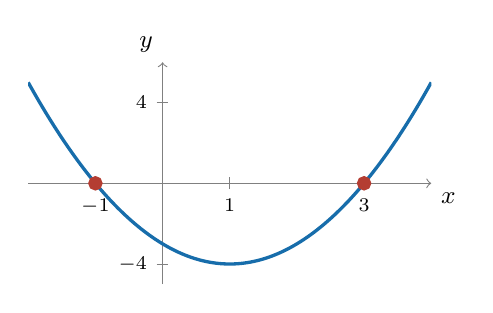
\begin{tikzpicture}
      \begin{axis}[lessonaxis,xmin=-2,xmax=4,ymin=-5,ymax=6,xtick={-1,0,1,3},ytick={-4,0,4}]
        \addplot[mathblue,domain=-2:4]{x^2-2*x-3};
        \addplot[only marks,mark=*,mathred] coordinates {(-1,0)(3,0)};
      \end{axis}
    \end{tikzpicture}
  \end{column}
  \end{columns}
  \src{一元二次方程的实数根，就是相应二次函数的零点。}
\end{frame}

\begin{frame}[t]{复习导入：这个方程怎样解}
  \large
  对于方程
  \[\ln x+2x-6=0,\qquad x>0,\]
  不能像一元二次方程那样，直接套用求根公式。
  \pause
  \gap
  能否借助函数
  \[y=\ln x+2x-6\]
  研究方程有没有实数解、解在什么范围内、有几个解？
\end{frame}

\begin{frame}[t]{新知探究：函数的零点}
  \large
  设函数 $y=f(x)$ 的定义域为 $D$。
  \begin{block}{零点}
    使 $f(x_0)=0$ 的实数 $x_0\in D$，叫作函数 $y=f(x)$ 的零点。
  \end{block}
  \gap
  \pause
  以 $f(x)=x^2-4$ 为例：
  \begin{itemize}
    \item 零点是\key{实数 $-2,2$}。
    \item 对应的图象交点是\key{$(-2,0),(2,0)$}。
    \item 对应的函数值都是\key{$0$}。
  \end{itemize}
  \src{湘教版必修第一册 4.4.1。}
\end{frame}

\begin{frame}[t]{新知探究：三种表述}
  \large
  对同一个实数 $x_0$：
  \[\boxed{x_0\in D,\ f(x_0)=0}\]
  \begin{align*}
    &\Longleftrightarrow\quad x_0\text{ 是方程 }f(x)=0\text{ 的实数根}\\[2mm]
    &\Longleftrightarrow\quad x_0\text{ 是函数 }y=f(x)\text{ 的零点}\\[2mm]
    &\Longleftrightarrow\quad (x_0,0)\text{ 是图象与 }x\text{ 轴的交点}.
  \end{align*}
  \pause
  \gap
  口答：$f(2)=0$ 时，零点是 $\underline{\qquad}$，交点是 $\underline{\qquad\qquad}$。
  \gap\key{答案：$2$；$(2,0)$。}
\end{frame}

\begin{frame}[t]{新知探究：河流情境}
  \centering
  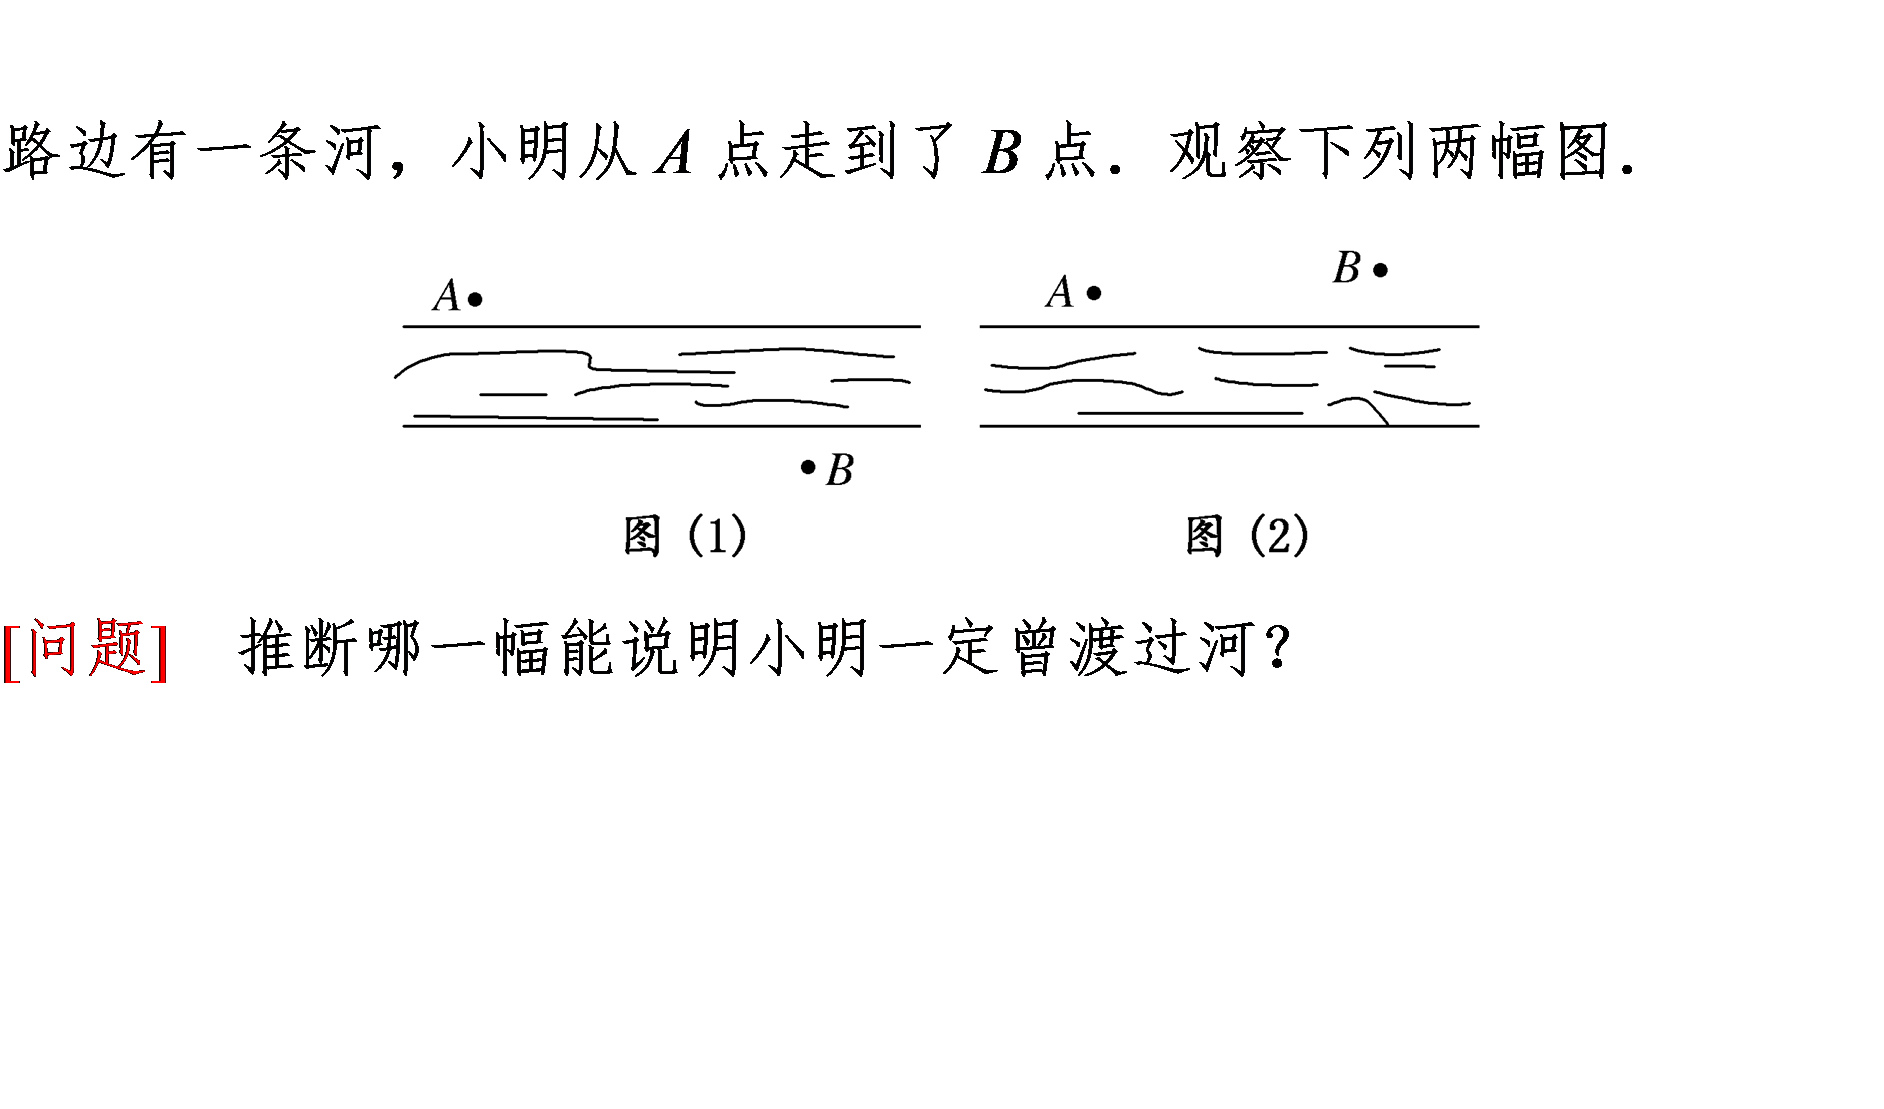
\includegraphics[trim=0 300bp 0 65bp,clip,width=13.7cm,height=4.6cm,keepaspectratio]{assets/原PPT第4页_河流情境.png}
  \pause
  \par\small\key{图（1）至少经过一次河流；图（2）不能保证经过。}
  \gap
  \small 假设路线连续、河流在讨论区域贯通，且不能绕过源头。
  \src{思考：把河流看作横轴，两岸分别对应函数值的正负。}
\end{frame}

\begin{frame}[t]{新知探究：观察函数图象}
  \begin{columns}[T,onlytextwidth]
  \begin{column}{.53\textwidth}
    \centering
    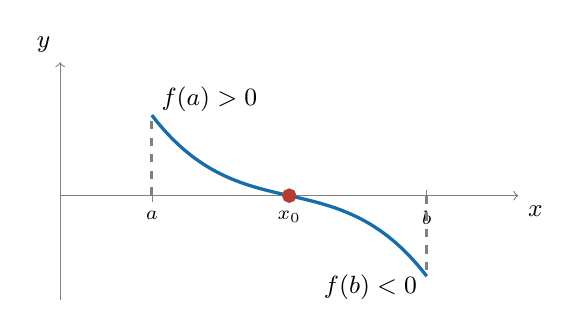
\begin{tikzpicture}\begin{axis}[lessonaxis,width=7.4cm,height=4.6cm,xmin=0,xmax=5,ymin=-2.5,ymax=3.2,xtick={1,2.5,4},xticklabels={$a$,$x_0$,$b$},ytick=\empty]
      \addplot[mathblue,domain=1:4]{-.35*(x-2.5)^3-.5*(x-2.5)};
      \addplot[dashed,gray] coordinates {(1,0)(1,1.93125)};
      \addplot[dashed,gray] coordinates {(4,0)(4,-1.93125)};
      \addplot[only marks,mathred] coordinates {(2.5,0)};
      \node[font=\small,anchor=west] at (axis cs:1,2.3){$f(a)>0$};
      \node[font=\small,anchor=east] at (axis cs:4,-2.2){$f(b)<0$};
    \end{axis}\end{tikzpicture}
  \end{column}
  \begin{column}{.44\textwidth}
    \large
    \begin{itemize}
      \item 图象连续不断。
      \gap
      \item 左端点在 $x$ 轴上方。
      \gap
      \item 右端点在 $x$ 轴下方。
    \end{itemize}
    \pause
    \gap 中间至少与 $x$ 轴相交一次。
    \gap\key{$f(a)f(b)<0$ 表示两端异号。}
  \end{column}
  \end{columns}
  \src{湘教版必修第一册 图4.4-1。}
\end{frame}

\begin{frame}[t]{新知探究：零点存在定理}
  \large
  \begin{block}{条件}
    设 $a<b$。函数 $y=f(x)$ 在闭区间 $[a,b]$ 上的图象\key{连续不断}，
    且 $\key{f(a)f(b)<0}$。
  \end{block}
  \pause
  \begin{block}{结论}
    在开区间 $(a,b)$ 内\key{至少有一个}零点。
    \[\text{即存在 }x_0\in(a,b),\quad f(x_0)=0.\]
  \end{block}
  \pause
  \gap
  \key{连续、异号}是使用条件；\key{开区间、至少一个}是结论关键词。
  \src{条件在闭区间 $[a,b]$ 上核查，结论落在开区间 $(a,b)$ 内。}
\end{frame}

\begin{frame}[t]{新知探究：连续性不可少}
  \begin{columns}[T,onlytextwidth]
  \begin{column}{.48\textwidth}
    \large $f(x)=\dfrac1x$。
    \[f(-1)=-1,\qquad f(1)=1.\]
    能推出 $(-1,1)$ 内有零点吗？
    \pause
    \gap\key{不能。}
    \gap $x=0$ 不在定义域内，图象在 $[-1,1]$ 上不连续。
    \gap 且 $\dfrac1x=0$ 没有实数解。
  \end{column}
  \begin{column}{.49\textwidth}
    \centering
    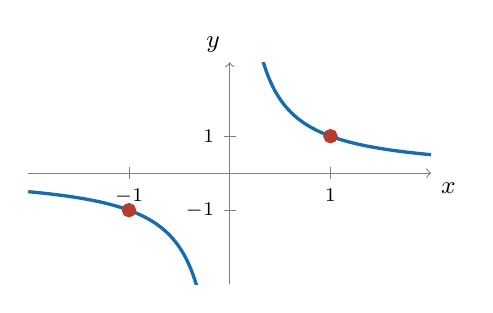
\begin{tikzpicture}\begin{axis}[lessonaxis,xmin=-2,xmax=2,ymin=-3,ymax=3,xtick={-1,1},ytick={-1,1}]
      \addplot[mathblue,domain=-2:-.15]{1/x};
      \addplot[mathblue,domain=.15:2]{1/x};
      \addplot[only marks,mathred] coordinates {(-1,-1)(1,1)};
    \end{axis}\end{tikzpicture}
  \end{column}
  \end{columns}
\end{frame}

\begin{frame}[t]{新知探究：同号与零点个数}
  \begin{columns}[T,onlytextwidth]
  \begin{column}{.49\textwidth}
    \centering\key{同号，也可能有零点}
    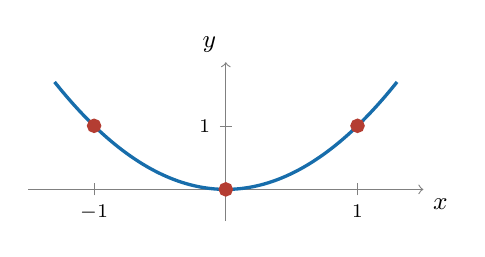
\begin{tikzpicture}\begin{axis}[lessonaxis,width=6.6cm,height=3.6cm,xmin=-1.5,xmax=1.5,ymin=-.5,ymax=2,xtick={-1,0,1},ytick={1}]
      \addplot[mathblue,domain=-1.3:1.3]{x^2};
      \addplot[only marks,mathred] coordinates {(-1,1)(0,0)(1,1)};
    \end{axis}\end{tikzpicture}
    \par $f(x)=x^2$，$f(-1)f(1)>0$。
    \par 零点为 $0$。
  \end{column}
  \begin{column}{.49\textwidth}
    \centering\key{异号，可能有多个零点}
    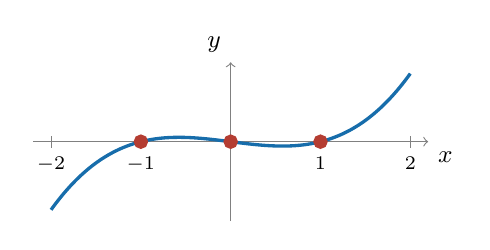
\begin{tikzpicture}\begin{axis}[lessonaxis,width=6.6cm,height=3.6cm,xmin=-2.2,xmax=2.2,ymin=-7,ymax=7,xtick={-2,-1,0,1,2},ytick=\empty]
      \addplot[mathblue,domain=-2:2]{x^3-x};
      \addplot[only marks,mathred] coordinates {(-1,0)(0,0)(1,0)};
    \end{axis}\end{tikzpicture}
    \par $g(x)=x^3-x=x(x-1)(x+1)$。
    \par $g(-2)g(2)<0$，却有3个零点。
  \end{column}
  \end{columns}
  \pause\gap\centering\large 定理给出\key{存在的充分条件}，并不确定恰有几个。
\end{frame}

\begin{frame}[t]{新知探究：零点的唯一性}
  \large
  \begin{align*}
    \text{连续且端点异号}&\quad\Longrightarrow\quad \text{\key{至少一个}；}\\[3mm]
    \text{在该区间严格单调}&\quad\Longrightarrow\quad \text{\key{至多一个}。}
  \end{align*}
  \pause
  \[\text{存在性与唯一性结合，才能说明恰有一个零点。}\]
  \gap
  若严格递增，$x_1<x_2$ 时 $f(x_1)<f(x_2)$，不可能同时为 $0$。
  \pause
  \gap
  反问：$y=2^x$ 严格递增，一定有零点吗？
  \gap\key{没有。严格单调本身只说明“至多一个”。}
\end{frame}

\begin{frame}[t]{新知探究：定理的应用}
  \large
  讨论 $f(x)=2x^3-5$ 在 $(1,2)$ 内零点的个数。
  \pause
  \gap
  \key{存在性：}函数在 $[1,2]$ 上连续，且
  \[f(1)=-3<0,\qquad f(2)=11>0.\]
  所以在 $(1,2)$ 内\key{至少有一个}零点。
  \pause
  \gap
  \key{唯一性：}$x^3$ 严格递增，所以 $2x^3-5$ 严格递增。
  故在 $(1,2)$ 内\key{至多有一个}零点。
  \gap
  综上，在 $(1,2)$ 内\key{恰有一个}零点。
  \src{湘教版必修第一册 4.4.1 例1。}
\end{frame}

\begin{frame}[t]{课堂练习：求函数零点}
  \large
  求下列函数的零点：
  \par（1）$f(x)=x^2+7x+6$；
  \par（2）$g(x)=1-\log_2(x+3)$。
  \pause
  \gap
  （1）定义域为 $\mathbb R$。
  \[f(x)=0\ \Longleftrightarrow\ (x+1)(x+6)=0.\]
  零点为\key{$-1,-6$}。
  \pause
  \gap
  （2）定义域为 $(-3,+\infty)$。
  \[g(x)=0\ \Longleftrightarrow\ \log_2(x+3)=1
    \ \Longleftrightarrow\ x=-1.\]
  $-1>-3$，所以零点为\key{$-1$}。
  \src{先看定义域，再解 $f(x)=0$，最后检验。}
\end{frame}

\begin{frame}[t]{课堂练习：分式函数}
  \large
  求函数 $f(x)=\dfrac{x^2+4x-12}{x-2}$ 的零点。
  \gap
  \pause
  \key{先保留原定义域：$x\ne2$。}
  \[f(x)=\frac{(x+6)(x-2)}{x-2}=x+6\qquad(x\ne2).\]
  \pause
  \[f(x)=0\ \Longleftrightarrow\ x=-6.\]
  所以函数只有一个零点，零点为\key{$-6$}。
  \gap
  \alert{$x=2$ 使分子为 $0$，但原函数在这里没有定义。}
  \src{《三维设计》必修第一册（人教A版适用），第77页。}
\end{frame}

\begin{frame}[t]{课堂练习：分段函数}
  \large
  求函数 $f(x)=\begin{cases}x^2+2x-3,&x\le0,\\-2+\ln x,&x>0\end{cases}$ 的零点。
  \pause
  \gap
  当 $x\le0$ 时，$(x+3)(x-1)=0$，候选根为 $-3,1$。
  \gap 因为 $1$ 不满足 $x\le0$，只保留\key{$-3$}。
  \pause
  \gap
  当 $x>0$ 时，$\ln x=2$，得到\key{$x=e^2$}，满足该段范围。
  \gap
  因此函数有\key{两个零点：$-3,e^2$}。
  \src{《三维设计》必修第一册（人教A版适用），第77页典例3。}
\end{frame}

\begin{frame}[t]{课堂练习：方程根的区间}
  \large
  判断方程 $\ln x+2x-6=0$ 的解的个数，并确定它所在的相邻整数区间。
  \pause
  \gap
  令 $f(x)=\ln x+2x-6$，定义域为 $(0,+\infty)$。
  \[f(2)=\ln2-2<0,\qquad f(3)=\ln3>0.\]
  函数在 $[2,3]$ 上连续，所以在 $(2,3)$ 内至少有一个零点。
  \pause
  \gap
  $\ln x$ 与 $2x$ 在 $(0,+\infty)$ 上都严格递增，故 $f$ 严格递增。
  \gap
  因此原方程恰有一个实数解，且在 $(2,3)$ 内。
  \src{由 $\ln2<1$ 可知 $\ln2-2<0$。本题无需算出精确根。}
\end{frame}

\begin{frame}[t]{课堂练习：判断零点区间}
  \large
  不求精确值，判断 $f(x)=2^x+\log_2x-3$ 的零点所在区间。
  \pause
  \gap
  \key{第一步：定义域为 $(0,+\infty)$，选取易算的端点。}
  \[f(1)=2+0-3=-1,\qquad f(2)=4+1-3=2.\]
  \pause
  \key{第二步：在 $[1,2]$ 上连续，且端点异号。}
  \gap 因此在 $(1,2)$ 内至少有一个零点。
  \pause
  \gap
  \key{第三步：若要确定唯一，还需性质。}
  \gap $2^x$、$\log_2x$ 在定义域上都严格递增，因此 $f$ 严格递增。
  \gap 所以函数在整个定义域内\key{只有一个零点，位于 $(1,2)$}。
  \src{《三维设计》必修第一册（人教A版适用），第77页。}
\end{frame}

\begin{frame}[t]{课堂练习：根据数值表判断}
  \large
  二次函数 $f(x)=ax^2+bx+c\ (a\ne0)$ 的部分函数值如下。
  不求系数，判断两个零点所在的区间。
  \gap\centering
  \begin{tabular}{c|rrrrrrrr}\toprule
    $x$&$-3$&$-2$&$-1$&$0$&$1$&$2$&$3$&$4$\\\midrule
    $f(x)$&$6$&$m$&$-4$&$-6$&$-6$&$-4$&$n$&$6$\\\bottomrule
  \end{tabular}
  \pause
  \gap\raggedright
  $f(-3)f(-1)<0$，$f(2)f(4)<0$。
  \gap 二次函数连续，因此两个区间\key{$(-3,-1)$、$(2,4)$}内各至少一个。
  \pause
  \gap 二次函数至多有两个不同零点，所以两区间内\key{各恰有一个}。
  \src{《三维设计》必修第一册（人教A版适用），第77页典例2。}
\end{frame}

\begin{frame}[t]{课堂练习：两图象的交点}
  讨论方程 $2^{-x}=\log_2x$ 的解的个数与所在区间。
  \begin{columns}[T,onlytextwidth]
  \begin{column}{.55\textwidth}
    \centering
    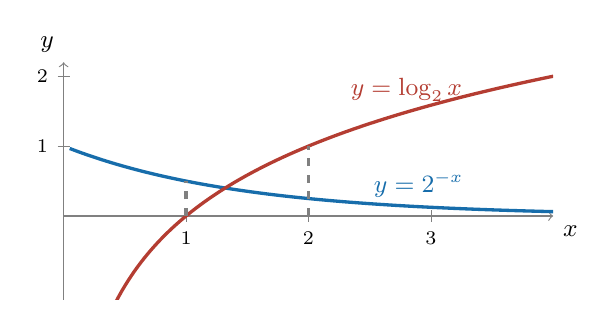
\begin{tikzpicture}\begin{axis}[lessonaxis,width=7.8cm,height=4.6cm,xmin=0,xmax=4,ymin=-1.2,ymax=2.2,xtick={1,2,3},ytick={1,2}]
      \addplot[mathblue,domain=.05:4]{2^(-x)};
      \addplot[mathred,domain=.4:4]{ln(x)/ln(2)};
      \node[mathblue,font=\small] at (axis cs:2.9,.45){$y=2^{-x}$};
      \node[mathred,font=\small] at (axis cs:2.8,1.8){$y=\log_2x$};
      \addplot[dashed,gray] coordinates {(1,0)(1,.5)};
      \addplot[dashed,gray] coordinates {(2,0)(2,1)};
    \end{axis}\end{tikzpicture}
  \end{column}
  \begin{column}{.42\textwidth}
    \large
    定义域的共同部分为 $x>0$。
    \gap
    $2^{-x}$ 严格递减，$\log_2x$ 严格递增。
    \pause
    \gap
    观察可知，交点的横坐标在 $(1,2)$ 内，且至多有一个交点。
    \gap
    用函数的性质说明这个判断。
  \end{column}
  \end{columns}
  \src{湘教版必修第一册 4.4.1 例2。}
\end{frame}

\begin{frame}[t]{课堂练习：零点个数的论证}
  \large
  令 $h(x)=\log_2x-2^{-x}$，定义域为 $(0,+\infty)$。
  \pause
  \gap
  \key{存在性：}$h$ 在 $[1,2]$ 上连续，且
  \[h(1)=-\frac12<0,\qquad h(2)=1-\frac14=\frac34>0.\]
  所以 $h$ 在 $(1,2)$ 内至少有一个零点。
  \pause
  \gap
  \key{唯一性：}$\log_2x$ 严格递增，$-2^{-x}$ 也严格递增，
  因而 $h$ 在\key{整个定义域}上严格递增。
  \gap
  所以原方程\key{恰有一个实数解，且在 $(1,2)$ 内}。
  \src{唯一性应在整个定义域上说明，才能排除区间外其他根。}
\end{frame}

\begin{frame}[t]{课堂练习：绝对值与零点}
  \large
  已知 $f(x)=|x^2-4x|-a$ 恰有3个零点，求 $a$。
  \pause
  \gap
  \[f(x)=0\quad\Longleftrightarrow\quad |x^2-4x|=a.\]
  即研究 $y=|x^2-4x|$ 与水平直线 $y=a$ 的交点。
  \gap
  先画 $y=x^2-4x=(x-2)^2-4$，把 $x$ 轴下方部分沿 $x$ 轴翻折。
  \gap
  \key{关键位置：$(0,0),(2,4),(4,0)$。}
  \src{《三维设计》必修第一册（人教A版适用），第77页。}
\end{frame}

\begin{frame}[t]{课堂练习：交点个数}
  \begin{columns}[T,onlytextwidth]
  \begin{column}{.55\textwidth}
    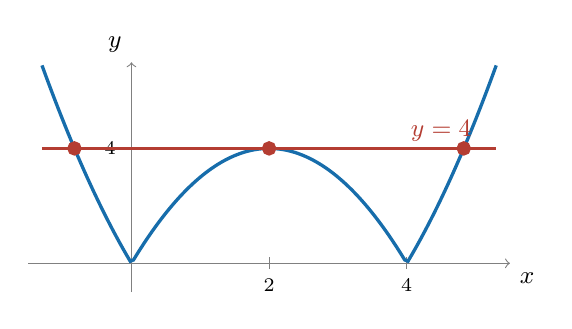
\begin{tikzpicture}\begin{axis}[lessonaxis,width=7.7cm,height=4.5cm,xmin=-1.5,xmax=5.5,ymin=-1,ymax=7,xtick={0,2,4},ytick={4}]
      \addplot[mathblue,domain=-1.3:5.3]{abs(x^2-4*x)};
      \addplot[mathred,domain=-1.3:5.3]{4};
      \addplot[only marks,mathred] coordinates {(-.828427,4)(2,4)(4.828427,4)};
      \node[mathred,font=\small] at (axis cs:4.5,4.6){$y=4$};
    \end{axis}\end{tikzpicture}
  \end{column}
  \begin{column}{.42\textwidth}
    \large
    \begin{tabular}{c|c}
      $a$ 的范围 & 交点数\\\hline
      $a<0$ & 0\\
      $a=0$ & 2\\
      $0<a<4$ & 4\\
      $a=4$ & 3\\
      $a>4$ & 2
    \end{tabular}
    \pause
    \gap\key{因此 $a=4$。}
    \gap\small 此时 $(x-2)^2=8$ 或 $0$，
    零点是 $2-2\sqrt2,2,2+2\sqrt2$。
  \end{column}
  \end{columns}
  \src{当 $a=4$ 时，方程有三个不同实根。}
\end{frame}

\begin{frame}[t]{课堂练习：两根分居两侧}
  \large 设 $f_a(x)=x^2-2ax+4$。
  若两个零点满足 $x_1<1<x_2$，求 $a$ 的范围。
  \begin{columns}[T,onlytextwidth]
  \begin{column}{.51\textwidth}
    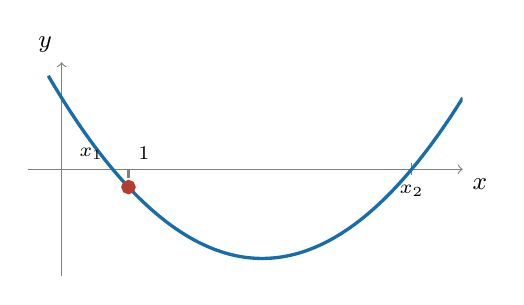
\begin{tikzpicture}\begin{axis}[lessonaxis,width=7.1cm,height=4.3cm,xmin=-.5,xmax=6,ymin=-6,ymax=6,xtick={5.236068},xticklabels={$x_2$},ytick=\empty]
      \addplot[mathblue,domain=-.2:6]{x^2-6*x+4};
      \addplot[dashed,gray] coordinates {(1,0)(1,-1)};
      \addplot[only marks,mathred] coordinates {(1,-1)};
      \node[font=\scriptsize,anchor=south east] at (axis cs:.763932,0){$x_1$};
      \node[font=\scriptsize,anchor=south west] at (axis cs:1,0){$1$};
    \end{axis}\end{tikzpicture}
  \end{column}
  \begin{column}{.46\textwidth}
    \gap\large
    开口向上。
    \gap
    $1$ 在两个零点之间，对应图象在 $x$ 轴下方。
    \pause
    \gap
    \key{$f_a(1)<0$。}
  \end{column}
  \end{columns}
  \src{图中取 $a=3$ 示意。}
\end{frame}

\begin{frame}[t]{课堂练习：两根分居两侧}
  \large
  \[f_a(1)=5-2a<0\quad\Longleftrightarrow\quad\key{a>\frac52}.\]
  \pause
  \gap
  为什么这一条足够？
  \begin{itemize}
    \item 开口向上，点 $(1,f_a(1))$ 在 $x$ 轴下方；
    \item 抛物线左右两端最终都在 $x$ 轴上方；
    \item 所以在 $1$ 左右各有一个零点，且二次函数至多有两个。
  \end{itemize}
  \pause
  \gap
  \key{一般结论：}对 $f(x)=Ax^2+Bx+C\ (A\ne0)$，
  \[x_1<t<x_2\quad\Longleftrightarrow\quad\boxed{A f(t)<0}.\]
  \src{这里的条件已保证两个不同实根。开口向下时，$f(t)$ 的符号相反。}
\end{frame}

\begin{frame}[t]{课堂练习：两根均大于1}
  \large 仍设 $f_a(x)=x^2-2ax+4$，要求 $1<x_1<x_2$。
  \begin{columns}[T,onlytextwidth]
  \begin{column}{.51\textwidth}
    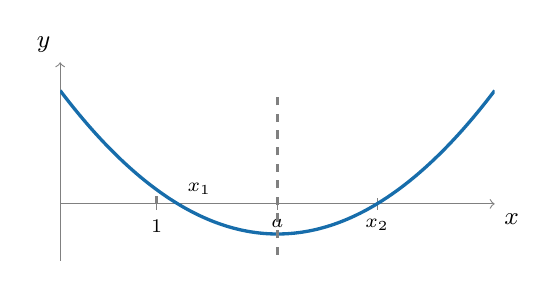
\begin{tikzpicture}\begin{axis}[lessonaxis,width=7.1cm,height=4.1cm,xmin=0,xmax=4.5,ymin=-2,ymax=5,xtick={1,2.25,3.280776},xticklabels={$1$,$a$,$x_2$},ytick=\empty]
      \addplot[mathblue,domain=0:4.5]{x^2-4.5*x+4};
      \addplot[dashed,gray] coordinates {(1,0)(1,.5)};
      \addplot[dashed,gray] coordinates {(2.25,-1.8)(2.25,4)};
      \node[font=\scriptsize,anchor=south west] at (axis cs:1.219224,0){$x_1$};
    \end{axis}\end{tikzpicture}
  \end{column}
  \begin{column}{.46\textwidth}
    \pause\large
    三个位置条件缺一不可：
    \gap\par\key{$\Delta>0$：}确有两个不同零点。
    \gap\par\key{$a>1$：}对称轴在 $1$ 右侧。
    \gap\par\key{$f_a(1)>0$：}$1$ 在两根外侧。
  \end{column}
  \end{columns}
  \src{示意图取 $a=9/4$。仅凭 $f_a(1)>0$，两根也可能都在左侧，或根本没有实根。}
\end{frame}

\begin{frame}[t]{课堂练习：两根均大于1}
  \large
  \[\begin{cases}
    \Delta=4a^2-16>0,\\
    a>1,\\
    f_a(1)=5-2a>0
  \end{cases}
  \quad\Longleftrightarrow\quad\boxed{2<a<\frac52}.\]
  \pause
  \gap
  \key{端点检验}
  \par $a=2$ 时，$f_a(x)=(x-2)^2$，只有一个不同零点。
  \gap
  \par $a=\dfrac52$ 时，$f_a(x)=(x-1)(x-4)$，有一个零点等于 $1$。
  \gap 两个端点都不能取。
  \src{《三维设计》必修第一册（人教A版适用），第77页典例4改编。}
\end{frame}

\begin{frame}[t]{课堂练习：两根均在区间内}
  \large
  已知 $f_m(x)=x^2-2mx+2$，两个不同零点都在 $(0,3)$ 内，求 $m$ 的范围。
  \pause
  \gap
  结合开口向上的抛物线，依次检查：
  \[\begin{cases}
      \Delta>0, &\text{有两个不同零点},\\
      0<m<3, &\text{对称轴在区间内},\\
      f_m(0)>0,\ f_m(3)>0, &\text{两端点在根的外侧}.
    \end{cases}\]
  \gap
  \key{只写两端点函数值大于0，还不能保证区间内有两个零点。}
  \src{说明判别式、对称轴和端点符号三个方面各自的作用。}
\end{frame}

\begin{frame}[t]{课堂练习：两根均在区间内}
  \large
  \[\begin{cases}
    4m^2-8>0,\\
    0<m<3,\\
    f_m(0)=2>0,\\
    f_m(3)=11-6m>0
  \end{cases}
  \quad\Longleftrightarrow\quad\boxed{\sqrt2<m<\frac{11}{6}}.\]
  \pause
  \gap
  $m=\sqrt2$ 时，判别式为 $0$，两个根重合。
  \gap
  $m=\dfrac{11}{6}$ 时，$f_m(3)=0$，一个根落到端点 $3$。
  \gap 因此两个端点都排除。
\end{frame}

\begin{frame}[t]{课堂练习：两个指定区间}
  \large
  $f_a(x)=x^2-2ax+4$ 的一个零点在 $(0,1)$ 内，另一个在 $(6,8)$ 内，求 $a$。
  \pause
  \gap
  开口向上，$1,6$ 都在两根之间，$0,8$ 在两根外侧。
  \[\begin{cases}
    f_a(0)=4>0,\\
    f_a(1)=5-2a<0,\\
    f_a(6)=40-12a<0,\\
    f_a(8)=68-16a>0
  \end{cases}
  \quad\Longleftrightarrow\quad\boxed{\frac{10}{3}<a<\frac{17}{4}}.\]
  \pause
  \gap
  两个不相交区间内各至少一个零点，二次函数又至多有两个，故各恰有一个。
  \src{《三维设计》必修第一册（人教A版适用），第77页典例4。}
\end{frame}

\begin{frame}[t]{课堂练习：综合练习}
  \large
  \par（1）求 $2x^2-x-1$ 的零点。
  \gap
  \par（2）$f(x)=x^3-8$ 在 $(1,3)$ 内有几个零点？写出理由。
  \gap
  \par（3）“连续函数在区间两端同号，区间内就没有零点。”判断并举例。
  \pause
  \gap\hrule\gap
  （1）$(2x+1)(x-1)=0$，零点为\key{$-\frac12,1$}。
  \par（2）连续、$f(1)=-7<0,f(3)=19>0$，且严格递增，\key{恰有一个}。
  \par（3）错误，如\key{$f(x)=x^2$ 在 $[-1,1]$ 上}。
  \src{（1）（2）据湘教版必修第一册本节练习改编。}
\end{frame}

\begin{frame}[t]{课堂小结：零点问题的方法}
  \large
  \begin{tabular}{p{3.4cm}p{9.4cm}}\toprule
    问题 & 方法\\\midrule
    求零点 & 解 $f(x)=0$，检验定义域。\\[3mm]
    判断所在区间 & 函数连续，端点异号，得出区间内存在零点。\\[3mm]
    判断零点个数 & 既说明有几个，又说明不会有更多。\\[3mm]
    二次函数零点分布 & 画草图，结合判别式、对称轴和端点符号。\\\bottomrule
  \end{tabular}
  \gap
  零点是实数。连续、异号保证至少一个；严格单调保证至多一个。
\end{frame}

\begin{frame}[t]{课堂小结：二次函数零点分布}
  \large
  对二次函数 $f(x)=Ax^2+Bx+C\ (A\ne0)$：
  \begin{tabular}{p{4.2cm}p{8.5cm}}\toprule
    零点位置 & 从草图提取的条件\\\midrule
    $x_1<t<x_2$ & $Af(t)<0$。\\[4mm]
    $t<x_1<x_2$ & $\Delta>0$，对称轴在 $t$ 右侧，$Af(t)>0$。\\[4mm]
    $p<x_1<x_2<q$ & $\Delta>0$，对称轴在 $(p,q)$ 内。\newline $Af(p)>0$，$Af(q)>0$。\\\bottomrule
  \end{tabular}
  \gap 每个条件都要与图象位置对应，最后检验端点。
  \src{表中均要求两个不同零点。区间含端点或允许重根时，必须重新分析等号。}
\end{frame}

\begin{frame}[t]{课堂小结：本课的数学素养}
  \large
  \begin{tabular}{p{2.4cm}p{10.3cm}}\toprule
    数学抽象 & 从二次函数推广到一般函数，用 $f(x_0)=0$ 刻画零点。\\[3mm]
    直观想象 & 用交点理解根与零点，用图象解释连续与异号。\\[3mm]
    逻辑推理 & 检查定理条件，区分至少、至多与恰有。\\[3mm]
    数学运算 & 解简单方程，计算端点函数值，检验定义域。\\\bottomrule
  \end{tabular}
  \gap
  用图象理解，用符号表达，用性质说明理由。
  \src{依据《普通高中数学课程标准（2017年版2025年修订）》。}
\end{frame}

\begin{frame}[t]{布置作业}
  \large
  \textbf{书面作业}
  \par（1）求 $x^3-x^2-4x+4$ 的零点。
  \par（2）求 $\log_2(x^2-2x-2)$ 的零点，并检验定义域。
  \gap
  \textbf{应用练习}
  \par（3）证明 $2^x+\lg(x+1)-2$ 有唯一零点，并确定它所在的相邻整数区间。
  \gap
  \textbf{根的分布}
  \par（4）已知 $x^2-2ax+4$ 的两个不同零点分居 $1$ 两侧，怎样判断 $a$？
  \src{（1）（2）湘教版教材本节练习；（3）（4）据往年课件及教辅改编。}
\end{frame}

\end{document}
